\documentclass[]{article}
\usepackage{polski}
\usepackage[utf8]{inputenc}
\usepackage{amsmath}
\usepackage{graphicx}
\usepackage{geometry}
\geometry{legalpaper, margin=0.5in}

%opening
\title{AMO - Projekt 1, zestaw 25}
\author{Jakub Postępski}

\begin{document}

\maketitle


\section{Układ równań współrzędnych kartezjańskich}
Dla każdego punktu w układzie współrzędnych "geograficznych" mamy:
\[ x = r\cos \theta \cos \phi \]
\[ y = r\cos \theta \sin \phi \]
\[ z = r\sin \theta \]
gdzie $ \theta $ to długość geograficzna i $ \phi $ to szerokość geograficzna.

Dla każdego punktu w układzie współrzędnych kartezjańskich mamy:
\[ r = \sqrt{x^2 + y^2 + z^2}\]
\[ \theta = \arctan \frac{y}{x} \]
\[ \phi = \arcsin \frac{z}{r} \]

Zakładamy, że czas dotarcia dla każdego satelity obarczony jest błędem $b_i$ oraz prędkość swiatła $c=299792458$ m/s.

Szukane współrzędne w układzie kartezjańskim punktu oznaczymy jako $x$, $y$ oraz $z$, a w układzie "geograficznym" jako $r$, $\theta$, $\phi$. Współrzędne satelit będziemy oznaczać z dolnymi indeksami odpowiadającymi numerowi satelity.


\section{Zadanie optymalizacji w układzie wsp. kartezjańskich} 
Należy zminiamalizować sumę kwadratów funkcji $f(x)$ wyrażających błąd pomiędzy zmierzonym a rzeczywistym czasem dotarcia sygnału z satelit do odbiornika.

\[ \min || f(x) ||^2_2 = \min (f(x_1)^2 + ... + f(x_5)^2)\]

dla funkcji:

\[ f(x_i) = \sqrt{(x-x_i)^2 + (y-y_i)^2 + (z-z_i)^2}-t_i*C\]

gdzie: 
\begin{itemize}
	\item $x$, $y$, $z$ to wsp. szukanego punktu
	\item $x_i$, $y_i$, $z_i$ to wsp. odpowiedniego satelity
	\item $t_i$ to zmierzony czas dotarcia sygnału z satelity
	\item $C$ to stała określająca prędkość światła
\end{itemize}

\section{Jakobian funkcji optymalizowanej}

\section{Rozwiązanie zadania}
Oba programy (Matlab oraz AMPL) wyznaczyły to samo położenie 
\[ \theta = 51.3759 , \phi = 21.3779 \] i tą samą wysokość nad poziomem morza ($172$ m).


\section{Zaburzanie wyniku}
Zaburzanie wyników wykonano w programie Matlab
\subsection{Czasu pojedynczego satelity}

\subsection{Wsp. pojedynczego satelity}
\subsection{Czasu wszystkich satelitów}
\subsection{Wsp. wszystkich satelitów}

\section{Zmiana parametrów solwera Matlaba}
Na początku zastosowano domyślny algorytm Trust Region Reflective, który zatrzymywał się po 22 iteracjach. Algorytm Levenberga-Marquardta (stosowany do dalszych badań) zatrzymał się po 5 iteracjach, co świadczy o jego znacznej przewadze.

\section{Google Maps}
\begin{figure}
	\centering
	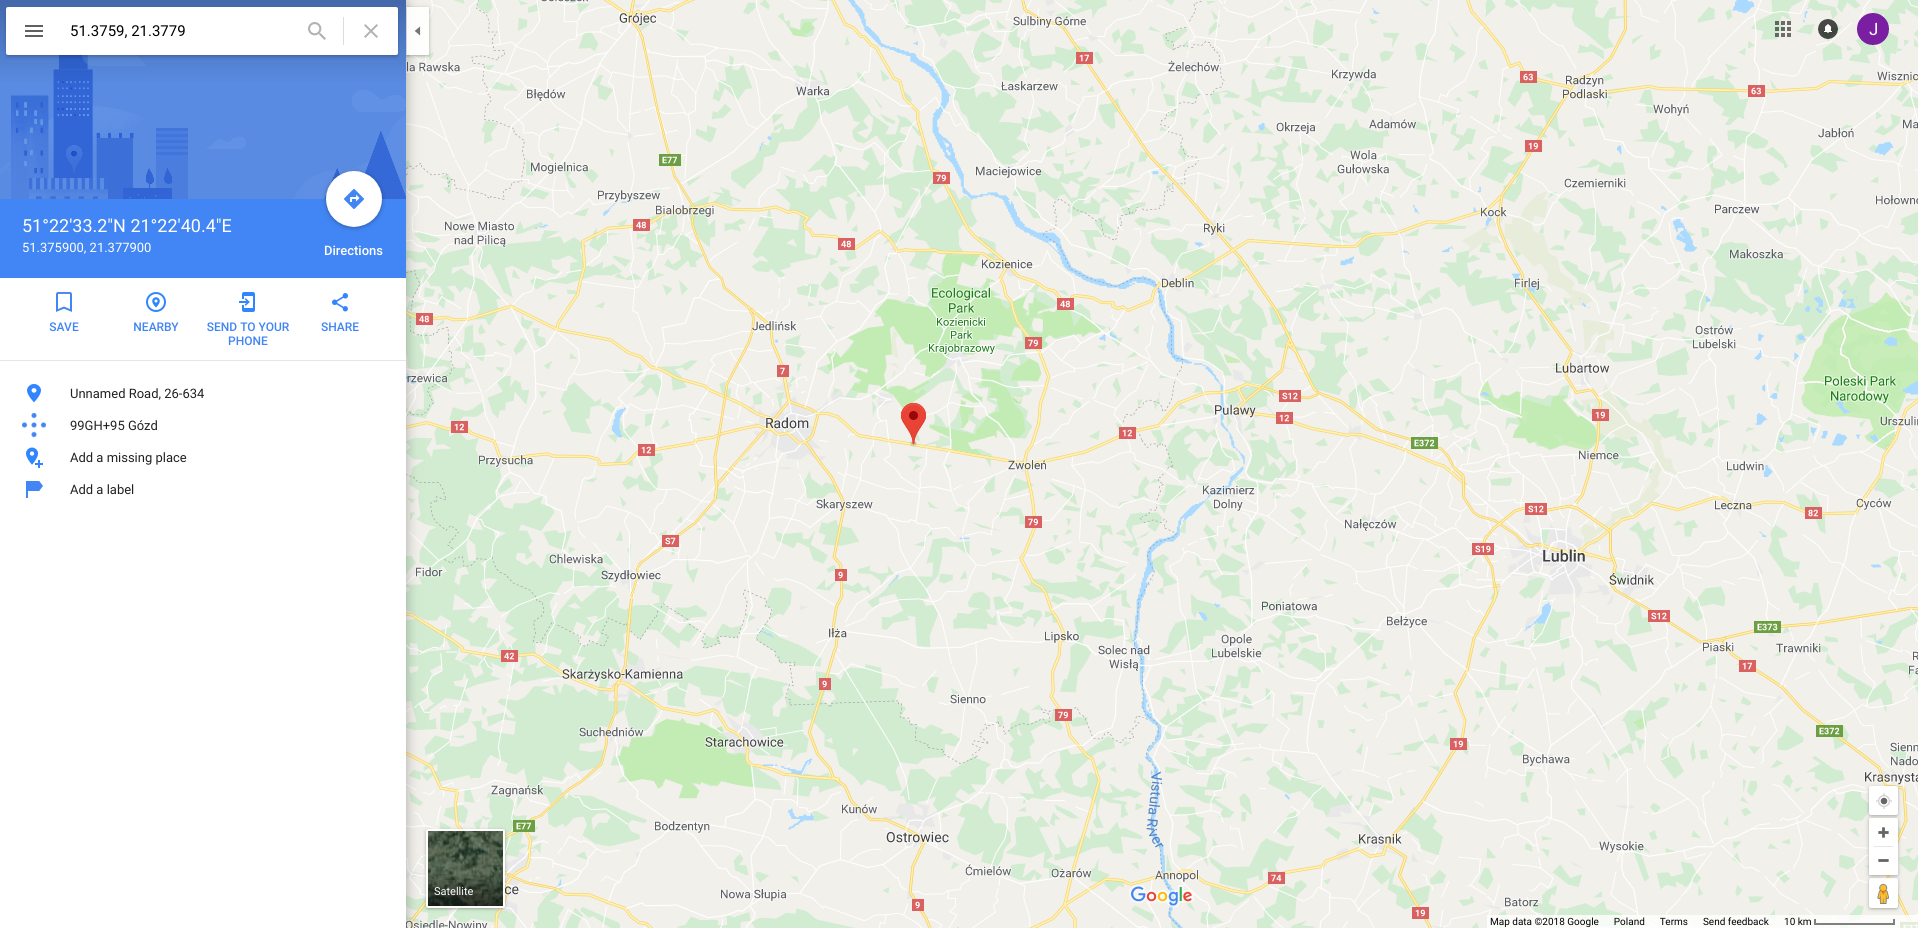
\includegraphics[width=0.99\linewidth]{daleko}
	\caption{Widok daleki znalezionego punktu}
	\label{fig:daleko}
\end{figure}

\begin{figure}
	\centering
	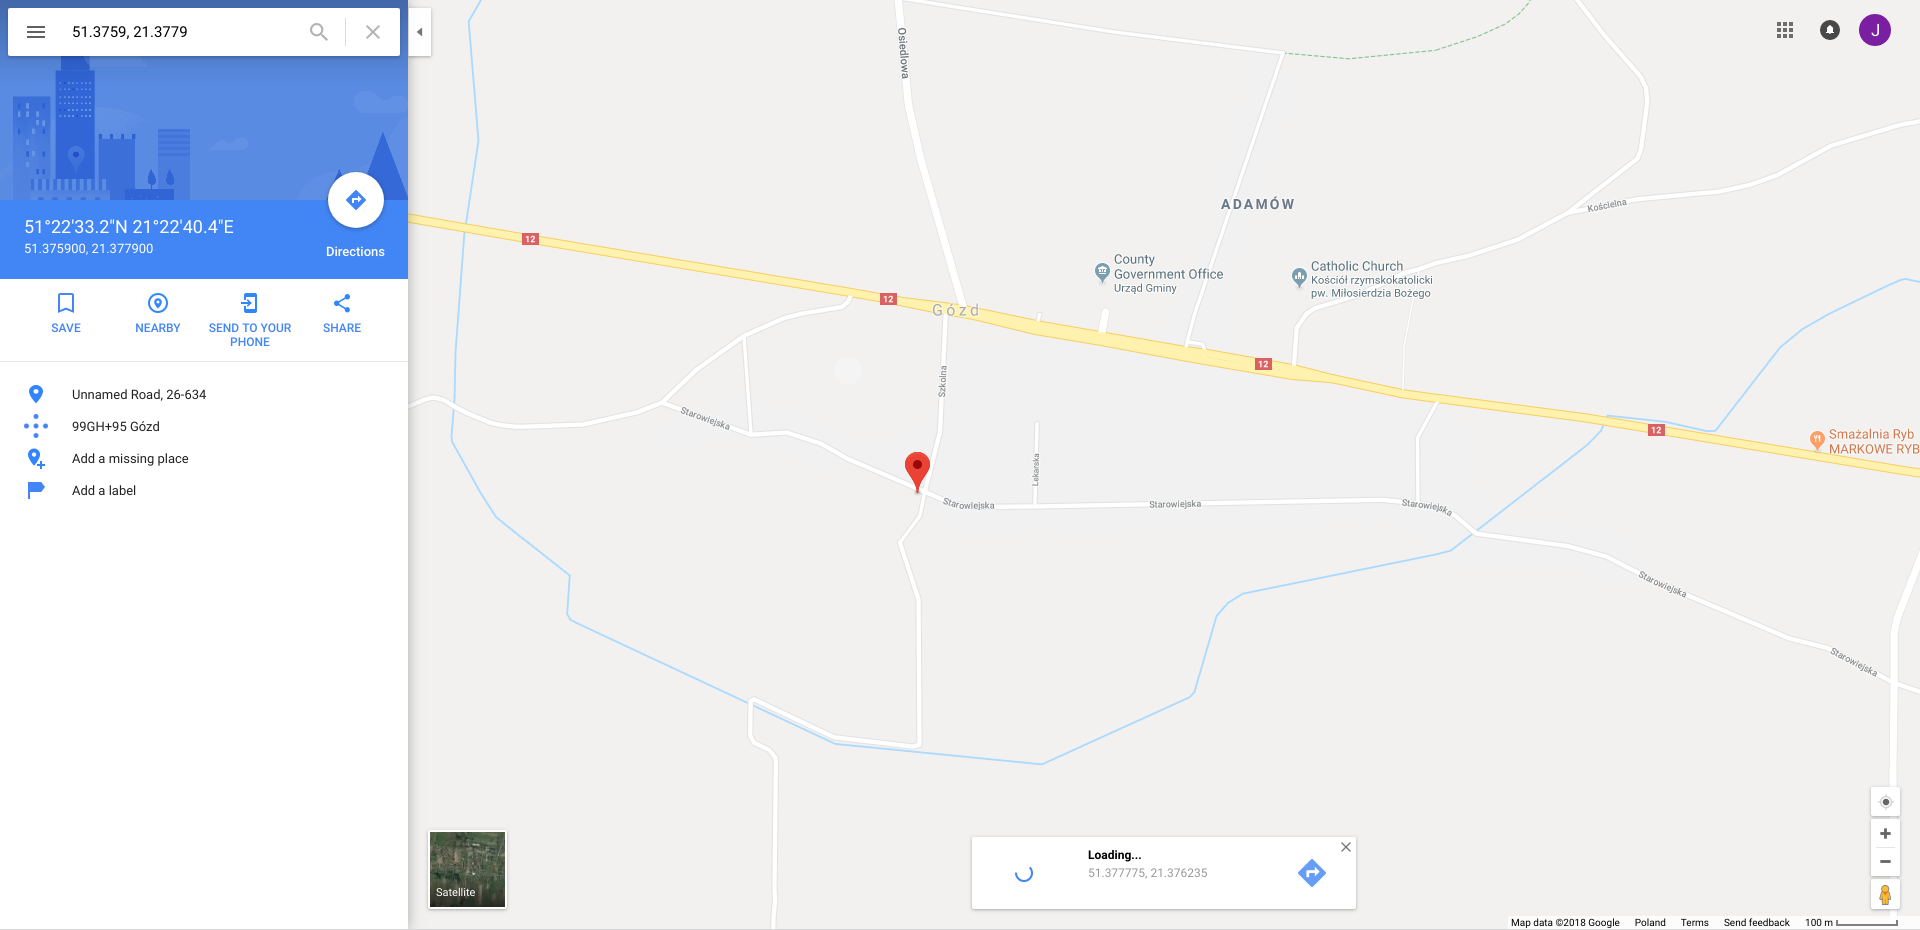
\includegraphics[width=0.99\linewidth]{blisko}
	\caption{Widok miejscowości znalezionego punktu}
	\label{fig:blisko}
\end{figure}


\end{document}
